% !TEX root = thesis.tex

%\section{Introduction}
%
%\begin{abstract}
%
%\end{abstract}
\tableofcontents
%\listoffigures

\clearpage
\section{Introduction}
\label{sec:introduction}
This thesis focuses on studying Quantum Chromodynamics (QCD)~\cite{gross1973asymptotically}, a part of the standard model of particle physics~\cite{Tanabashi:2018oca}, which is the theory describing the strong interactions. Strong interaction is the force responsible for interactions that holds the nucleus of an atom together. Fundamentally it describes the interactions between quarks and gluons, the elementary constituents of the building blocks of the nucleus, protons and neutrons. Because of specifics of this interaction quarks and gluons, together dubbed partons, can never be seen free~\cite{Perl:2004qc}. Under ordinary conditions they are confined into bound states called hadrons. In extreme conditions they can form a medium of asymptotically free quarks and gluons, guark-gluon plasma (QGP)~\cite{Shuryak:1980}. %Understanding QGP is the holy grail of heavy-ion physics

Indirectly partons can be observed in high energy particle collisions as jets, collimated showers of particles~\cite{Perkins:1982xb}. The physics of these jets is the primary topic discussed in this thesis. Understanding jets is important when one is interested in the processes that produce the partons that eventually fragment into jets. By themselves jets can provide an insight into QCD when the fragmentation is studied. Jets can also be used as probes of the QGP medium. 

Experimentally jets can be studied with jet reconstruction algorithms which group observed tracks, in essence undoing the showering process, to find a reasonable estimate of the initial parton. That is also the case in this thesis. The main observable studied is the jet fragmentation transverse momentum \jt{} which is defined as the perpendicular component of the momentum of jet constituents with respect to the jet axis, the best estimate of the initial parton. As such \jt{} measures the transverse nudge that fragmentation products receive.

The analysis studies collisions between protons and lead nuclei. Originally these were meant to be a reference for lead-lead collisions to rule out possible cold nuclear matter effects~\cite{Connors:2017ptx}; effects caused by the regular 'cold' nuclear matter of a nucleus as opposed to QGP. However, \pPb collisions have provided interesting physics by themselves. Many of the collective phenomena that in \PbPb collisions were attributed to QGP have been observed also in high multiplicity \pPb collisions~\cite{Nagle:2018nvi} and even in ultra high multiplicity \pp collisions~\cite{Nagle:2018nvi}. However observables of jet modification show no conclusive signals in \pPb collisions~\cite{Connors:2017ptx,Nagle:2018nvi}. %So far all observables have focused on 

This thesis is organised as follows: Section ~\ref{sec:introduction} first gives a general introduction into the history and properties of QCD and heavy-ion physics. It is followed by a description of hard processes, jet fragmentation and hadronisation and how these processes might look like in a heavy-ion environment. Finally there is a discussion on the physics of small systems.

The experimental setup that was used to collect the data in this thesis is described in Section ~\ref{sec:exp}. It starts by explaining the accelerator facilities at CERN and LHC in more detail. This is followed by a description of the ALICE experiment and its sub-detectors. A part of Section ~\ref{sec:exp} is dedicated to coming upgrades of ALICE as this is a timely topic. In 2019-2020 ALICE will be upgraded and I have made a personal contribution to the TPC upgrade.

Section ~\ref{sec:selection} gives a description of the event, track and cluster selection criteria used in the analysis. This is followed in Section ~\ref{sec:methods} by the specific analysis methods used in this thesis. First the jet reconstruction algorithm used, anti-\kt{}, is described. Section ~\ref{sec:methods} continues by introducing the \jt{} observable, how it is obtained and what methods are used to estimate background contribution and correct for detector effects. Finally the fitting method used for the final results is described. Section 5 gives the different systematic uncertainties that arise from the analysis.

Finally the results from the analysis are presented in Section ~\ref{sec:results}. The results are compared to \pythia~and Herwig Monte Carlo generators. Further discussion of the results is given in Section~\ref{sec:disc} when the results are compared to \jt{} results obtained with a different analysis method. Section~\ref{sec:sum} summarises the main results and gives an outlook for future.


\pagebreak
\subsection{Quantum chromodynamics}
\subsubsection{Foundation of QCD}
The universe is governed by four basic interactions: gravity, electromagnetic, weak and strong interactions. The standard model of particle physics~\cite{Tanabashi:2018oca} includes three of these, electromagnetic, weak and strong interactions.  The fourth one, gravity, is described well in all but the most extreme of cases by the theory of general relativity~\cite{Einstein1915}. The standard model is a quantum field theory where local gauge symmetries dictate  particle interactions~\cite{Perkins:1982xb}. 

The first interaction included in the standard model was the electromagnetic interaction. The foundations of quantum field theory and Quantum Electrodynamics (QED) were already laid out by the work by Dirac in 1927~\cite{doi:10.1098/rspa.1927.0039}. The full theory of QED was formulated in 1946-1949 by Tomonaga~\cite{Tomonaga:1946zz},  Schwinger~\cite{Schwinger:1948yj,Schwinger:1948yk} and Feynman~\cite{Feynman:1948fi}% and Dyson~\cite{Dyson:1949bp},
%for which they received the Nobel prize in physics in ~\

Motivated by the success of a quantum field theory approach for the electromagnetic interaction physicists started working on the remaining interactions. However, the weak and strong nuclear interactions proved more challenging to formulate~\cite{Krauss:2017}. In the end the weak interaction was unified with the electromagnetic interaction into the electroweak theory. The final theory was formulated by Glashow~\cite{Glashow:1970gm}, Salam~\cite{Salam:1964ry} and Weinberg~\cite{Weinberg:1967tq}.

The theory of strong interactions became to be known as Quantum Chromodynamics (QCD). The search for a theory of strong interactions began already after the formulation of QED and drew further inspiration when new particle accelerators were introduced in the 1950s. These were powerful enough to conduct particle physics research while before this the main source of particle physics had been the study of cosmic rays. From cosmic ray studies positrons, neutrons and muons had been discovered in the 1930s and charged pions were discovered in 1947~\cite{Occhialini:1987nr,Lattes:1947mx}. The neutral pion was discovered in 1950~\cite{Bjorklund:1950}.

These new accelerators included the Bevalac accelerator which was commissioned at the Lawrence Berkeley National Laboratory (LBNL) in 1954. Bevalac was followed by the Super Proton Synchrotron  (SPS) at CERN in 1959 and by the Alternating Gradient Synchrotron (AGS) at the Brookhaven National Laboratory (BNL) in 1960. The most powerful of these was the AGS which could reach energies of up to \unit[33]{\gev} with proton beams. With these accelerators a host of new particles were discovered by the beginning of the 1960s. The most notable were antiprotons~\cite{Chamberlain:1955ns}, antineutrons~\cite{Cork:1957nu}, $\Delta$-particles and the six hyperons ($\Xi^0$\cite{Alvarez:1959zz}, $\Xi^-$~\cite{Armenteros:1952nt}, $\Sigma^{\pm}$~\cite{Bonetti1953}, $\Sigma^0$~\cite{Plano1957} and $\Lambda$~\cite{Fowler:1953qpk}).


Physicists started searching for symmetries between these newly observed particles. Already in 1932 Heisenberg~\cite{Heisenberg:1932} had used an SU(2) symmetry in his isospin model to group protons and neutrons, as apart from electrical charge these behave almost identically. In 1962 this was extended by Gell-Mann and Ne'eman ~\cite{Gell-Mann:1962} to the SU(3) symmetry based organisation of particles. In this SU(3) model hadrons sharing the same spin and parity numbers were grouped into octets. This lead to the discovery of the $\Omega^{-}$~\cite{Barnes:1964ga} baryon as the SU(3) decouplet that included heavier baryons was missing a baryon. 

In the SU(3) symmetry group the simplest representation is a triplet where particles would have electric charges $\nicefrac{2}{3}$ or $-\nicefrac{1}{3}$. However, no particles with fractional charge had been detected. Although they still didn't consider these to be real particles, Gell-Mann~\cite{Gell-Mann:1964} and Zweig~\cite{Zweig:1964jf} proposed in 1964 that baryons and mesons would be bound states of these three hypothetical triplet particles. Now we know that these are the $u$, $d$ and $s$ quarks. The term quark was coined by Gell-Mann while Zweig had called them aces.

This original quark model still had a problem as it violated the Pauli exclusion principle. Because of the antisymmetry of fermion wave functions no two similar fermions can share the exact same quantum numbers. However, in a particle comprised of three identical (same flavour) quarks, like the $\Omega^{-}$ particle, at least two quarks would have the same quantum numbers, as the only variable quantum number, spin, can have two values for quarks with spin \nicefrac{1}{2}. This problem was solved by the addition of another quantum number, colour, which separated quarks of the same species. The idea of colour had been originally presented already in 1964 by Greenberg~\cite{Greenberg:1964}. A model combining quarks and colour was presented in 1971 by Gell-Mann and Fritzsch~\cite{Fritzsch:1972jv}. In the new colour model the baryonic wave function became

\begin{equation}
\left( qqq\right)\rightarrow\left(q_rq_gq_b-q_gq_rq_b+q_bq_rq_g-q_rq_bq_g+q_gq_bq_r-q_bq_gq_r\right),
\end{equation}

\noindent Experimentally the colour model could be confirmed by observables like the decay rate of a neutral pion and the Drell-Ratio. When taking colour into account the neutral pion decay rate is

\begin{equation}
\Lambda\left(\pi^0\rightarrow\gamma \gamma\right) = \frac{\alpha^2}{2\pi}\frac{N_c^2}{3^2}\frac{m_\pi^3}{f_\pi^2},
\end{equation} 

\noindent where $N_c$ is the number of colours. For $N_c=3$ this decay rate is \unit[7.75]{eV} while the measured value is $(7.86\pm0.54)\,\mathrm{eV}$~\cite{Williams:1988sg}.

The Drell-Ratio $R$~\cite{Krolikowski:1974jx} combines both the colour information and the number of quarks species. Defined as

\begin{equation}
R=\frac{\sigma\left(e^++e^-\rightarrow\mathrm{hadrons}\right)}{\sigma\left(e^++e^-\rightarrow\mu^++\mu^-\right)}=N_c\sum_fQ_f^2,
\end{equation}

\noindent this ratio has the numerical value 2 when the lightest quarks $u$, $d$ and $s$ are included. For collision energies exceeding the threshold of heavy quark ($c$ and $b$) production processes the ratio increases to $\nicefrac{10}{3}$ (for $f=u,d,s,c$) and \nicefrac{11}{3} (for $f=u,d,s,c,b$). So far the energy threshold ($\sqrt{s}\approx\unit[350]{\gev}$) of $t\bar t$ production, has not been reached by any $e^+e^-$ colliders.

%\cite{Glashow:1970gm} Introduction of lepton-quark symmetry by Glashow,Iliopoulos and Maiani, proposal of a fourth (charmed) quark.
%\\cite{Bacci:1974za} ADONE Discovery of charm quark and $J/\Psi$
%\cite{Aubert:1974js} BNL
%\cite{Augustin:1974xw} SLAC


In the colour model only colour neutral states are possible which explains why no free quarks had been observed. The simplest ways of producing a colour neutral object are the hadrons which can be observed, i.e. (anti)baryons and mesons, the combinations of either three (anti)quarks or a quark-antiquark pair respectively. Although the hunt for more exotic combinations has been going on for decades, only in 2019 did LHCb produce conclusive evidence of the observation of a pentaquark~\cite{Aaij:2019vzc}, a state which consists of 4 quarks and one antiquark.

First experimental indication of the existence of quarks came in 1969 when a series of experiments at the Stanford Linear Accelerator Center (SLAC) revealed that protons and neutrons appeared to have some substructure~\cite{Bloom:1969kc, Breidenbach:1969kd}. For this discovery they eventually received the Nobel Prize in Physics in 1990~\cite{Nobel1990}. Bjorken demonstrated that these results could be explained if protons and neutrons were composed of virtually noninteracting pointlike particles~\cite{Bjorken:1968dy,Bjorken:1969ja}. Feynman~\cite{Feynman:1969ej} interpreted these objects as real particles and suggested they would be the quarks of Gell-Mann's model. At the time, however, this seemed mysterious; if all strongly interacting particles, hadrons, were composed of quarks, then quarks should surely be strongly interacting themselves. Why would they appear to be almost free inside hadrons? This turned out to be a key clue in formulating the theory of strong interactions~\cite{Krauss:2017}.


With the inclusion of colour the final quantum field theory of QCD could be formed rapidly between 1972-1974. A significant contribution was the work done by Gross, Wilczek, Politzer and George for non-abelian gauge field theories~\cite{gross1973ultraviolet, politzer1973reliable, gross1973asymptotically, gross1974asymptotically, georgi1974electroproduction}. The work showed that quarks would indeed be asymptotically free in a non-abelian theory, which explained the results from SLAC. In 2004 Gross, Wilczek and Politzer received the Nobel Prize in Physics for their work~\cite{Nobel2004}. The role of gluons as the particles mediating the strong interaction was presented by Fritzsch, Gell-Mann and Leutwyler in 1973~\cite{fritzsch1973advantages}.

%Nobel1990 to Friedman, Kendall and Taylor for SLAC results
%Nobel1976 to Richter and Ting

The quark model was extended in 1974 when the discovery of the charm quark and the first charmed hadron, $J/\Psi$, was simultaneously published by teams from the SLAC~\cite{Augustin:1974xw}, from Brookhaven National Laboratory~\cite{Aubert:1974js} and from the ADONE collider in Frascati, Italy~\cite{Bacci:1974za}. In 1976 the Nobel Prize in Physics was awarded to Richter and Ting for the discovery of the charm quark~\cite{Nobel1976}. The existence of a fourth quark had already been speculated in 1964 by Bjorken and Glashow~\cite{Bjorken:1964gz}, but a proper prediction was provided by Glashow, Iliopoulos and Maiani in 1970~\cite{Glashow:1970gm} based on symmetries between leptons and quarks in weak interactions.

However, the mediating particles, gluons, had not been directly seen in any experiments. The existence could be inferred from observing that the quarks only carried about half of the momentum of protons~\cite{25gluons}. Direct evidence was first seen in 1979 at the Positron-Electron Tandem Ring Accelerator (PETRA) at DESY~\cite{Brandelik:1979bd, PhysRev.43.830, Berger1979418} in the form of a three jet event, where the third jet came from a gluon.

The two remaining quarks, bottom and top, were introduced by Kobayashi and Maskawa in 1973 to explain CP-violation~\cite{Kobayashi:1973fv}. For this they received the Nobel Prize in Physics in 2008~\cite{Nobel2008}. Bottom quark was discovered soon after, in 1977, at Fermilab~\cite{Herb:1977ek}. The heaviest quark, top quark, would eventually be discovered in 1995 by the CDF~\cite{Abe:1995hr} and DØ~\cite{Abachi:1994td} experiments at Fermilab.




\subsubsection{Asymptotic Freedom}
In Quantum Electrodynamics (QED) the vacuum becomes polarised in the vicinity of a charge. Virtual particle-antiparticle pairs populate the surroundings of the centre charge.
%Virtual particles with opposite charge are attracted, and virtual particles with like charge are repelled by the original charge. 
The net effect is that the field at any finite distance is partially cancelled. Closer to the central charge one sees less of the vacuum effect and the effective charge increases. With increasing distance to the charge the effective charge weakens until the QED coupling constant reaches the fine-structure constant $\alpha=\frac{1}{137}$~\cite{Perkins:1982xb}.

%The net effect is to partially cancel out the field at any finite distance. Getting closer and closer to the central charge, one sees less and less of the effect of the vacuum, and the effective charge increases.

%In Quantum Electrodynamics (QED) the electric charge is screened. In the vicinity of a charge, the vacuum becomes polarized. Virtual charged particle-antiparticle pairs around the charge are arranged so that opposing charges face each other. Since the pairs also include an equal amount opposite charge compared to the original charge the average charge seen by an observer at a distance is smaller. 


There is screening also in QCD because of the colour charges. However, as QCD is a non-abelian theory gluons can interact also with other gluons. The mediating particles of QED, photons, are neutral and thus can't interact with other photons. The self-interaction of gluons leads to the antiscreening of the colour charge which dominates over the screening effect. As the distance to the central charge increases, virtual gluons of the vacuum cause the coupling constant to grow larger. If the distance between colour charges, quarks, gets large enough the interaction is strong enough to produce a new quark-antiquark pair. Thus no free colour charges can be seen. On the other hand, at very small distances the coupling constant approaches zero. This is known as asymptotic freedom~\cite{Perkins:1982xb}.

%Contrary to QED, QCD is a non-abelian theory. In other words the generators of the symmetry group of QCD, SU(3), do not commute. This has the practical consequence that gluons interact also with other gluons, whereas in QED the neutral carrier particles, photons, only interact with charged particles.
%There is screening also in QCD because of the colour charges, but in addition to that there is antiscreening because of the gluon interactions. In QCD the antiscreening effect dominates over screening. Thus for larger distances to the colour charge the coupling constant is larger. This explains why no free colour charges can be observed. When the distance between charges increases the interaction strengthens until it is strong enough to produce a new quark-antiquark pair. On the other hand, at very small distances the coupling constant approaches zero. This is called asymptotic freedom~\cite{Perkins:1982xb}.

Extending the idea of asymptotic freedom Collins predicted in 1975~\cite{Collins:1975} a state where individual quarks and gluons would no longer be bound to hadrons. This state of bulk QCD matter, which can be seen as a separate phase of hadronic matter, was later coined Quark-Gluon Plasma (QGP) by Edward Shuryak in 1980~\cite{Shuryak:1980}. With some assumptions a phase diagram of hadronic matter can be drawn. Figure~\ref{fig:QCDphase} shows a schematic view of this phase diagram.

\begin{figure}[htb]
\centering
%\includegraphics[width=0.9\textwidth]{pics/qcd_ms_high}
\includegraphics[width=0.9\textwidth]{pics/QCDphase2.pdf}
\caption[QCD phase diagram]{A schematic illustration of the phase diagram of QCD matter. The $x$-axis, showing the quark chemical potential $\mu$, represents the imbalance between quarks and antiquarks. Along the $x$-axis the temperature is zero. Along the vertical axis the temperature increases, which takes us through the crossover from a hadronic gas to quark-gluon plasma. With low $\mu$ this is the regime explored by high-energy heavy-ion colliders and also the trajectory taken by the universe as it cooled after the Big Bang. The conditions in neutron stars correspond to the lower right corner, with low $T$ and high $\mu$. Figure from~\cite{Rajagopal:2001}.} %Permission needed?
\label{fig:QCDphase}
\end{figure}


At a time of $10^{-6}\mathrm{s}$ after the Big Bang the conditions in the early universe preferred the existence of QGP instead of hadronic matter. Nowadays the properties of QGP can be explored in laboratories, through collisions of heavy atomic nuclei at ultra-relativistic energies. The phase transition between QGP and ordinary hadronic matter is the only phase transition in a quantum field theory that can be studied by any current or foreseeable technology. Thus the study of QGP in extreme conditions is of high interest.

One important property of QGP is the shear viscosity to entropy ratio, $\eta/s$. It is believed that among all substances in nature this ratio has a universal minimum value of $1/4\pi \approx 0.08$. In the strong coupling of certain gauge theories this is reached~\cite{Kovtun:2004de}. Figure~\ref{fig:etas} shows the temperature dependance of $\eta/s$ for several substances. For all cases the $\eta/s$ ratio has a minimum value in the vicinity of the critical temperature, $T_c$~\cite{PhysRevLett.98.092301}. Therefore studying the $\eta/s$ ratio in QGP matter could also probe the critical point of QCD matter.

In $\sqrt{s_{NN}}=\unit[200]{\gev}$ Au--Au collisions at RHIC $\eta/s$ has been estimated to be $0.09\pm0.015$~\cite{PhysRevLett.98.092301}, which suggests that at least at some point during the evolution the matter is close to the critical point of QCD.

\begin{figure}[htb]
\centering
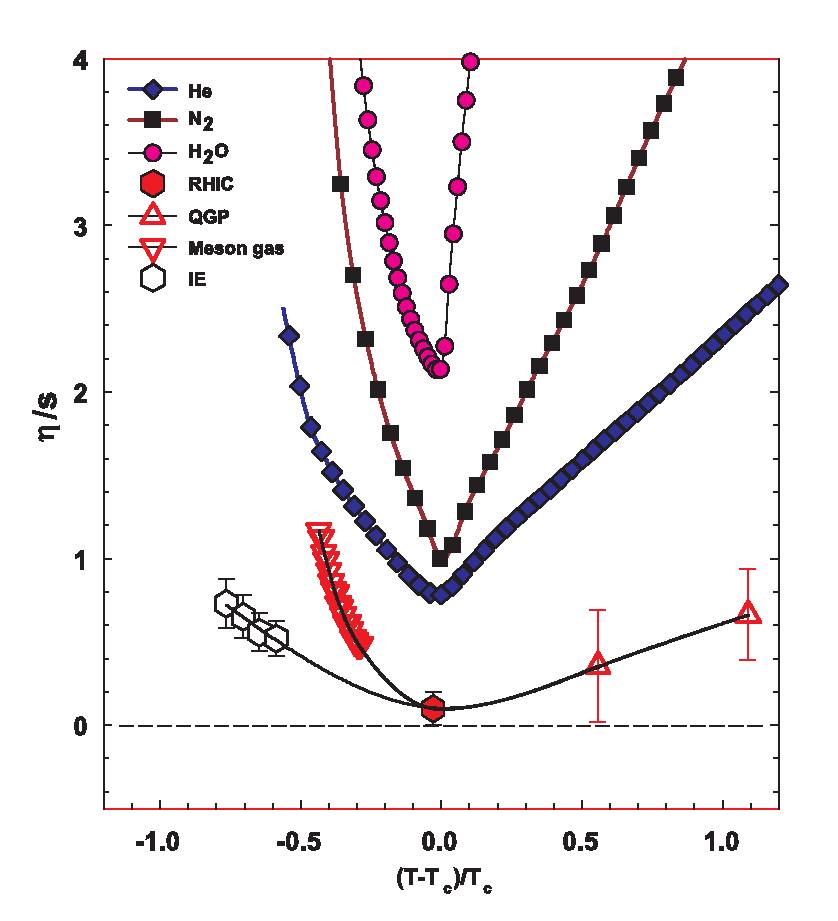
\includegraphics[width=0.9\textwidth]{pics/eta-s-vs-t-tc3}
\caption[$\eta/s$ vs $(T-T_c)/T_c$]{The figure shows \label{fig3}$\eta/s$ as a function of $(T-T_c)/T_c$ for several substances as indicated. The lines are drawn to guide the eye. The $\eta/s=0.09\pm0.015$ value at RHIC is estimated from Au--Au collisions at $\sqrt{s_{NN}}=\unit[200]{\gev}$. The calculations assume a value $T_c = \unit[170]{\mev}$ for nuclear matter. Figure from~\cite{PhysRevLett.98.092301}.
}
%Permission asked
\label{fig:etas}
\end{figure}



\FloatBarrier
\pagebreak
\subsection{Heavy-ion physics}
Quark Gluon Plasma (QGP) can be experimentally studied by colliding heavy-ions at high energies. Nowadays research of heavy-ion collisions is mainly performed at two particle colliders; The Relativistic Heavy-Ion Collider (RHIC) at BNL in New York, USA and the Large Hadron Collider (LHC) at CERN in Switzerland. Energy densities at these colliders are assumed to be large enough to produce QGP and indeed convincing evidence of QGP has been seen at both colliders. Complimentary research with heavy nuclei is also performed at the Super Proton Synchrotron (SPS) at CERN.

%The history of heavy-ion physics is strongly connected to the development of particle colliders. Experimental study of relativistic heavy-ion collisions has been carried out for three decades, beginning with the Bevalac at Lawrence Berkeley National Laboratory (LBNL)~\cite{Lofgren_1975}, and continuing with the AGS at Brookhaven National Laboratory (BNL)~\cite{Barton:1987}, CERN SPS~\cite{Vitev:2002pf}, culminating today with RHIC at BNL and LHC at CERN. 
%
%%The first colliders could not produce enough energy to create QGP matter so they could only probe the hadronic state. 
%%
%%The collective motion of matter in a heavy-ion collision has been modeled using several models e.g. the Blast wave Model~\cite{PhysRevC.84.064905} has been used succesfully. Another model growing in popularity is the hydrodynamical approach which is further discussed in section \ref{sec:hydro}.
%
%\subsubsection{History}
The first heavy-ion collisions were performed in fixed target experiments at the Bevalac experiment at the Lawrence Berkeley National Laboratory~\cite{Lofgren_1975} and at the Joint Institute for Nuclear Research in Dubna~\cite{kovalenko1994status}, which reached energies of up to \unit[1]{\gev} per nucleon. These were followed in 1986 by the Super Proton Synchrotron (SPS) at CERN which collided oxygen beams with fixed lead targets reaching a centre-of-mass energy per colliding nucleon pair $\left(\sqrt{s_{NN}}\right)$ of \unit[19.4]{\gev}~\cite{Vitev:2002pf}. However, no decisive evidence of QGP was found in these initial experiments. In 1994 SPS introduced a heavier lead beam to produce \PbPb collisions at $\sqrt{s_{NN}}\approx \unit[17]{\gev}$. Simultaneously the Alternating Gradient Synchrotron (AGS) at BNL started colliding ions like $\mathrm{^{32}S}$ with a fixed target at energies of up to \unit[28]{\gev}~\cite{Barton:1987}. In 2000 CERN~\cite{SPSpress} presented compelling evidence for the existence of a new state of matter in SPS. Today SPS is used for fixed-target experiments with \unit[400]{\gev} proton beams. One of these is the SPS heavy-ion and Neutrino Experiment (SHINE)~\cite{Grebieszkow:2013nza}, which tries to search for the critical point of strongly interacting matter.

The next significant addition was the Relativistic Heavy-Ion Collider (RHIC) at BNL in New York, USA which started operating in 2000 and keeps operating to this day. Instead of using fixed targets, RHIC can collide two accelerated beams, significantly increasing the potential centre-of-mass energy. In Au--Au collisions RHIC can reach a centre-of-mass energy per nucleon pair of \unit[200]{\gev}. The experiments at RHIC have provided a lot of convincing evidence that QGP was created~\cite{Adcox:2004mh, Adams:2005dq, Arsene:2004fa, Back:2004je}. 

The newest addition to the group of heavy-ion accelerators is the Large Hadron Collider (LHC) at CERN, Switzerland. Primarily used for proton-proton collisions LHC started operating in November 2009. A year later, in November 2010, first \PbPb heavy-ion runs began at $\sqrt{s_{NN}}=2.76\; \mathrm{TeV}$. Since then LHC has provided both \PbPb and \pPb collisions and a short period of Xe--Xe collisions. Table~\ref{tab:datasets} shows a summary of these. Among the main experiments at LHC, ALICE (a Large Ion Collider Experiment) is dedicated to heavy-ion physics. The all-purpose nature of CMS (Compact Muon Solenoid) and ATLAS (a Toroidal LHC Apparatus) make them well suited also for many heavy-ion studies and they have active heavy-ion programs. The fourth main experiment, LHCb, uses its SMOG system~\cite{Maurice:2017iom} to perform unique fixed target collisions with heavy ions, complementing the other experiments. 


\begin{table}[htb]
\centering
\caption{Summary of datasets. The integrated luminosities are from ALICE.}
\label{tab:datasets}
\begin{tabular}{| c | S | c |}
\hline
\multicolumn{3}{| c |}{Run 1 (2009-2013)} \\
\hline
\multirow{4}{*}{\pp} & 0.9 \tev & $\sim \unit[200]{\mu b^{-1}}$ \\
 & 2.76 \tev & $\sim \unit[100]{n b^{-1}}$ \\
 & 7.0 \tev & $\sim \unit[1.5]{p b^{-1}}$ \\
 & 8.0 \tev & $\sim \unit[2.5]{p b^{-1}}$ \\
 \hline
\pPb & 5.02 \tev & $\sim\unit[15]{n b^{-1}}$ \\
\hline
\PbPb & 2.76 \tev & $\sim \unit[75]{\mu b^{-1}}$ \\
\hline
\end{tabular}
\begin{tabular}{| c | S | c |}
\hline
\multicolumn{3}{| c |}{Run 2 (2015-2018)} \\
\hline
\multirow{2}{*}{\pp} & 5.02 \tev & $\sim \unit[1.3]{p b^{-1}}$ \\
 & 13.0 \tev & $\sim \unit[25]{p b^{-1}}$ \\
 \hline
\multirow{2}{*}{\pPb} & 5.02 \tev & $\sim\unit[3]{n b^{-1}}$ \\
& 8.16 \tev & $\sim\unit[25]{n b^{-1}}$ \\
\hline
Xe--Xe & 5.44 \tev & $\sim \unit[0.3]{\mu b^{-1}}$ \\
\hline
\PbPb & 5.02 \tev & $\sim \unit[1]{n b^{-1}}$ \\
\hline
\end{tabular}
\end{table}

\pagebreak
\FloatBarrier
%\pagebreak
\subsection{Features of heavy-ion collisions}
\label{sec:features}
\subsubsection{Collision Geometry}
\label{sec:geometry}
Since atomic nuclei have a significant transverse size, a collision between nuclei has geometric properties that provide insight into the collision dynamics.  One illustration of a heavy-ion collision is shown in Figure~\ref{fig:planes}. The main defining parameter of a collision is the vector connecting the centres of the two colliding nuclei at their closest approach, which is known as the impact parameter $\vec b$.

The impact parameter with the beam direction defines the reaction plane, which has an angle $\Psi_{RP}$ in the experimental reference frame, which is fixed by the detector setup. This reaction plane angle can be estimated with the event plane method~\cite{Voloshin:2008dg} since particle production changes as a function of the angle with respect to the reaction plane. 
\begin{figure}[h!]
\centering
%\definecolor{primary}{HTML}{0000FF}
%\definecolor{secondary}{HTML}{FF8000}
%\definecolor{tertiary}{HTML}{00FFFF}
%\begin{tikzpicture}
%      \draw[->] (-4,0) -- (4,0) node[below] {$x$};
%      \draw[->] (0,-3) -- (0,3) node[left] {$y$};
%       \coordinate[] (C);
% \coordinate[left=1cm of C] (C1);
%\coordinate[right=1cm of C] (C2);
%\draw[dashed, thick, primary] (C1) circle (2cm);
%\draw[dashed, thick, secondary] (C2) circle (2cm);
%      
%\end{tikzpicture}
\documentclass[border=5mm]{standalone}
\usepackage{tikz}
\usetikzlibrary{positioning}
\usetikzlibrary{intersections, calc, fadings}
\begin{document}
\definecolor{primary}{HTML}{0000FF}
\definecolor{secondary}{HTML}{FF8000}
\definecolor{tertiary}{HTML}{00FFFF}


\begin{tikzpicture}[scale=1]
      \draw[->,black!50] (-5.5,0) -- (5.5,0) node[below] {$x$};
      \draw[->,black!50] (0,-4) -- (0,4) node[left] {$y$};
       \coordinate[] (C);
 \coordinate[below left=0.5cm and 1.7cm of C] (C1);
\coordinate[above right=0.5cm and 1.7cm of C] (C2);
\coordinate[below left =1.5cm and 5.1cm of C] (D1);
\coordinate[above right =1.5cm and 5.1cm of C] (D2);

\coordinate[above left =3.4cm and 1.0cm of C] (D3);
\coordinate[below right =3.4cm and 1.0cm of C] (D4);

\draw[->,black!50] (D1) -- (D2) node[above] {$x_\mathrm{RP}$};
\draw[->,black!50] (D4) -- (D3) node[left] {$y_\mathrm{RP}$};

\draw[dashed, thick, primary] (C1) circle (3cm);
\draw[dashed, thick, secondary] (C2) circle (3cm);
\draw[->,thick] (C1) -- node[below right] {$\vec b$} (C2);
\draw[->] (1.5, 0) arc  (0:8.2:1.5cm) node[right] {$\Psi_\mathrm{RP}$} arc (8.2:16.4:1.5cm) ;


\end{tikzpicture}
\end{document}
%\includegraphics[width=0.6\textwidth]{pics/Definitions}
\caption[The definitions of the Reaction Plane coordinate systems]{The definition of the impact parameter and the reaction plane. The $x$--$y$ plane represents a coordinate system fixed by the experiment. The dashed circles are the two colliding nuclei. $x_{RP}$ is the reaction plane and $\Psi_\mathrm{RP}$ gives its angle.} %The angle between $x_{RP}$ and $x_{PP}$ is given by Eq. (\ref{eq:partangle}). $y_{PP}$ and $y_{RP}$ are lines perpendicular to the participant and reaction planes. }
\label{fig:planes}
\end{figure}

Although the length of the impact parameter can be used to quantise the centrality of a heavy-ion collisions in theoretical models, it is not practical in an experimental setup. Any connections between $\vec b$ and experimental observables is model-dependent. For a comparison of results between different experiments and models, one needs a general definition for centrality.

In practice this definition is provided by dividing events into percentile bins by the observed multiplicity of produced particles. In a heavy-ion collision the total multiplicity can be related to the number of participants. Small centrality percentages correspond to central events with the highest multiplicity while peripheral collisions have lower multiplicities and thus higher centrality percentages. Figure~\ref{fig:centrality} shows an observed multiplicity distribution from ALICE measurements~\cite{PhysRevC.88.044909} with the centrality bin division. The distribution is fitted using a phenomenological approach based on a Glauber Monte Carlo calculation~\cite{Miller:2007ri}.

\begin{figure}[tb]
\centering

               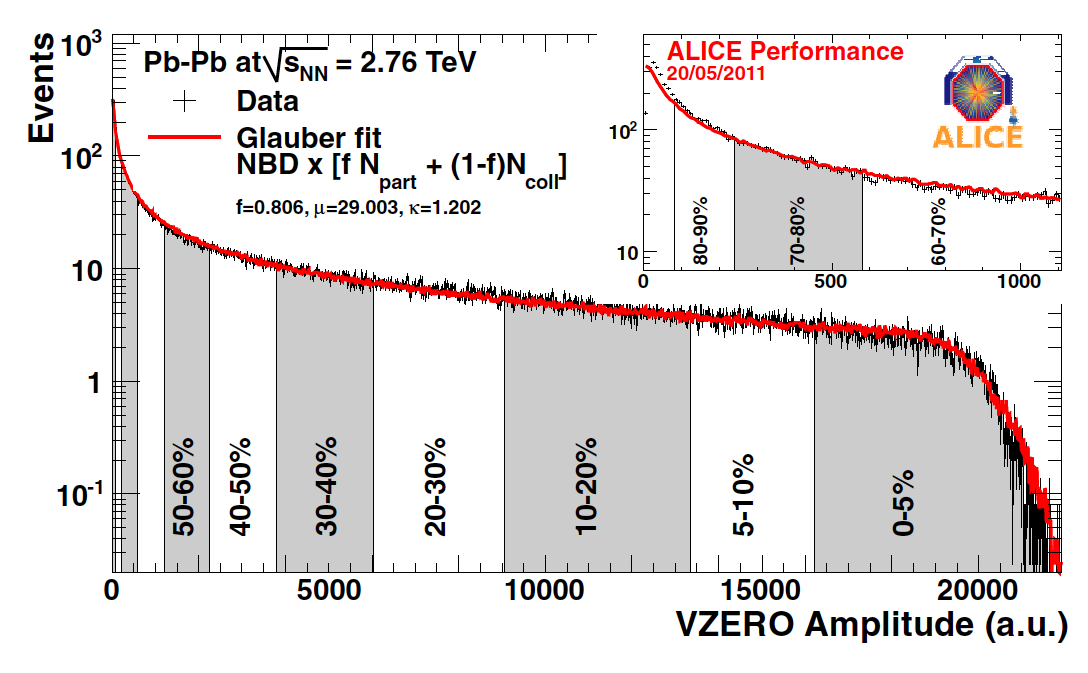
\includegraphics[width=0.9\textwidth]{pics/centrality.png}
        \caption[An illustration of the multiplicity distribution in ALICE measurement with centrality classes.]{An illustration of the multiplicity distribution which is divided into centrality bins in ALICE measurements. The red line shows the fit of the Glauber calculation to the measurement. Figure from~\cite{PhysRevC.88.044909}.}
        %Creative commons license
        	\label{fig:centrality}
\end{figure}


The Glauber Model is often used to model the nuclear geometry in a heavy-ion collision. The model was originally introduced already in 1958~\cite{Glauber:1959} and the modern terminology and tools were introduced in 1976 by Białłas, Bleszyński, and Czyż~\cite{Biallas1976461} to model inelastic nuclear collisions.


The model starts by defining the thickness function which is the integral of the nuclear density over a line going through the nucleus with minimum distance $s$ from the centre
of the nucleus
\begin{equation}
T_A\left(s\right)=\int_{-\infty}^{\infty}\dd z \rho\left(\sqrt{s^2+z^2}\right),
\end{equation}

\noindent where $ \rho\left(\sqrt{s^2+z^2}\right)$ is the number density of nuclear matter. This can be experimentally determined by studying the nuclear charge distribution in low-energy electron-nucleus scattering experiments~\cite{Miller:2007ri,DeJager:1987qc}. For a spherically symmetric nucleus a good approximation is given by the Woods-Saxon potential~\cite{Abelev:2013qoq}

\begin{equation}
\rho\left( r\right) = \frac{\rho_0 \left(1+\omega r^2 / R^2\right)}{1+\exp \left(\frac{r-R}{a}\right)},
\end{equation}


\noindent where $\rho_0$ is the nucleon density in the centre of the nucleus, $R$ is the nuclear radius, $a$ parametrizes the depth of the skin and $\omega$ can be used to introduce a surface excess. Figure~\ref{fig:woodssaxon} shows how this distribution looks like with parameters observed for lead nuclei. With $\omega=0$ the density changes only slightly as a function of $r$ until it quickly drops to almost 0 around $R$. The slope and length of the transition region is given by $a$. 

\begin{figure}
\centering
\begin{tikzpicture}
      \draw[->] (0,0) -- (7,0) node[below] {$r\left[\unit{fm}\right]$};
      \draw[->] (0,0) -- (0,5) node[left] {$\nicefrac{\rho}{\rho_0}$};
      \draw	(0,0) node[anchor=north] {0}
		(3,0) node[anchor=north] {5}
		(6,0) node[anchor=north] {10};

      \draw	(0,2) node[anchor=east] {0.5}
		(0,4) node[anchor=east] {1};
	
      \draw[dashed,black] (3.8,0) -- (3.8,5);

	
     \draw[black,thin,<->] (0,2) -- node[above] {$R$} (3.8,2);
     \draw[black,thin,<->] (3.55,1) -- node[below] {$a$} (4.05,1);
     
     \draw[blue] (2,3.5) node {$\omega=0$};
     \draw[blue] (2,4.5) node {$\omega>0$};

      \draw[scale=0.6,domain=0:10,smooth,variable=\x,blue,dashed] plot ({\x},{(6.66+1*\x^2/6.38^2)/(1+exp((\x-6.38)/0.546))});
       \draw[scale=0.6,domain=0:10,smooth,variable=\x,blue] plot ({\x},{(6.66)/(1+exp((\x-6.38)/0.546))});

      %\draw[scale=0.5,domain=-3:3,smooth,variable=\y,red]  plot ({\y*\y},{\y});

\end{tikzpicture}
\caption{Woods-saxon distribution, with typical values for a Pb nucleus, $a=0.55\unit{fm}$ and $R=6.6\unit{fm}$.}
\label{fig:woodssaxon}
\end{figure}


The integral over the overlap area of two thickness functions of colliding nuclei defines the overlap function 

\begin{equation}
T_{AB}\left(\vec b\right)=\int \dd{^2s} T_A\left(\vec s\right) T_B\left(\vec s - \vec b\right).
\end{equation}

\noindent In essence this is the material that takes part in the collision for a given impact parameter $\vec b$. The average overlap function, $\left<T_{AA}\right>$, in an A-A collisions  is given by~\cite{Afanasiev:2009aa}

\begin{equation}
\left<T_{AA}\right>=\frac{\int T_{AA}\left(b\right) \dd b}
{\int\left(1-e^{-\sigma^{inel}_{pp}T_{AA}\left(b\right)}\right)\dd b}.
\end{equation}

\noindent Using $\left<T_{AA}\right>$ one can calculate the mean number of binary collisions

\begin{equation}
\left<N_{coll}\right>=\sigma_{pp}^{inel}\left<T_{AA}\right>,
\end{equation}

\noindent where the total inelastic cross-section, $\sigma_{pp}^{inel}$, gives the probability of two individual nucleons interacting. As every binary collision has an equal probability for direct production of high-momentum particles the number of high momentum tracks is proportional to $\left<N_{coll}\right>$~\cite{Abelev:2013qoq,Kharzeev:2004if,Deng:2010mv}. This requires knowledge of $\sigma\mathrm{^{NN}_{inel}}$, which can be measured in proton-proton collisions with different energies. At the LHC the most precise cross section measurements come from TOTEM~\cite{Antchev:2017dia}.

Contrary to hard particles, soft particle production is based on the number of participants~\cite{Kharzeev:2004if}. It can be assumed that participating nucleons get excited and, since the time scales are too short for any reaction to happen in the nucleons, it does not matter how many interactions a single nucleon experiences. After the interactions excited nucleons produce a predictable number of soft particles. The average number of participants, $\left<N_{part}\right>$ can be calculated from the Glauber model  as


\begin{eqnarray}
\left<N_{part}^{AB}\left(\vec b\right)\right>&=&\int \dd{^2s} T_A\left(\vec s\right)\left[1-\left[1-\sigma_{NN}\frac{T_B\left(\vec s - \vec b\right)}{B}\right]^B\right] \nonumber \\
 &+ &\int \dd{^2 s} T_B\left(\vec s\right)\left[1-\left[1-\sigma_{NN}\frac{T_A\left(\vec s - \vec b\right)}{A}\right]^A\right].
\end{eqnarray}



In practice the Glauber model can be implemented in two common ways. Simple analytical expression can be obtained from the optical approximation. These include the nucleus-nucleus interaction cross-section, the number of interacting  nucleons and the number of nucleon-nucleon collisions on average. In the optical Glauber it is assumed that  the nucleons move independently during the crossing of the nuclei and they will be essentially undeflected.  

With increased appreciation for the physics emerging from fluctuations in the collision geometry the Glauber Monte Carlo (GMC) approach has provided a way to get a better  description of heavy-ion collisions. In GMC nucleons are distributed randomly according to the nuclear density distribution~\cite{Abelev:2013qoq}. In the simplest model nucleons of two nuclei will interact if their distance in the orthogonal plane, $d$ is small enough, i.e. 

%A heavy-ion collision is then treated as a series of independent nucleon-nucleon collisions, where in the simplest model nucleons interact if their distance  in the plane orthogonal to the beam axis, $d$, satisfies

\begin{equation}
d< \sqrt{\sigma\mathrm{^{NN}_{inel}}}.
\end{equation}

\noindent The number of participants and binary collisions can be calculated per event.  By simulating many heavy-ion collisions one can then determine both average values and the fluctuation around the average. The results of one GMC \PbPb event with impact parameter $b=\unit[9.8]{fm}$ is shown in Figure~\ref{fig:GMC}.

\begin{figure}[htbp]
\centering
               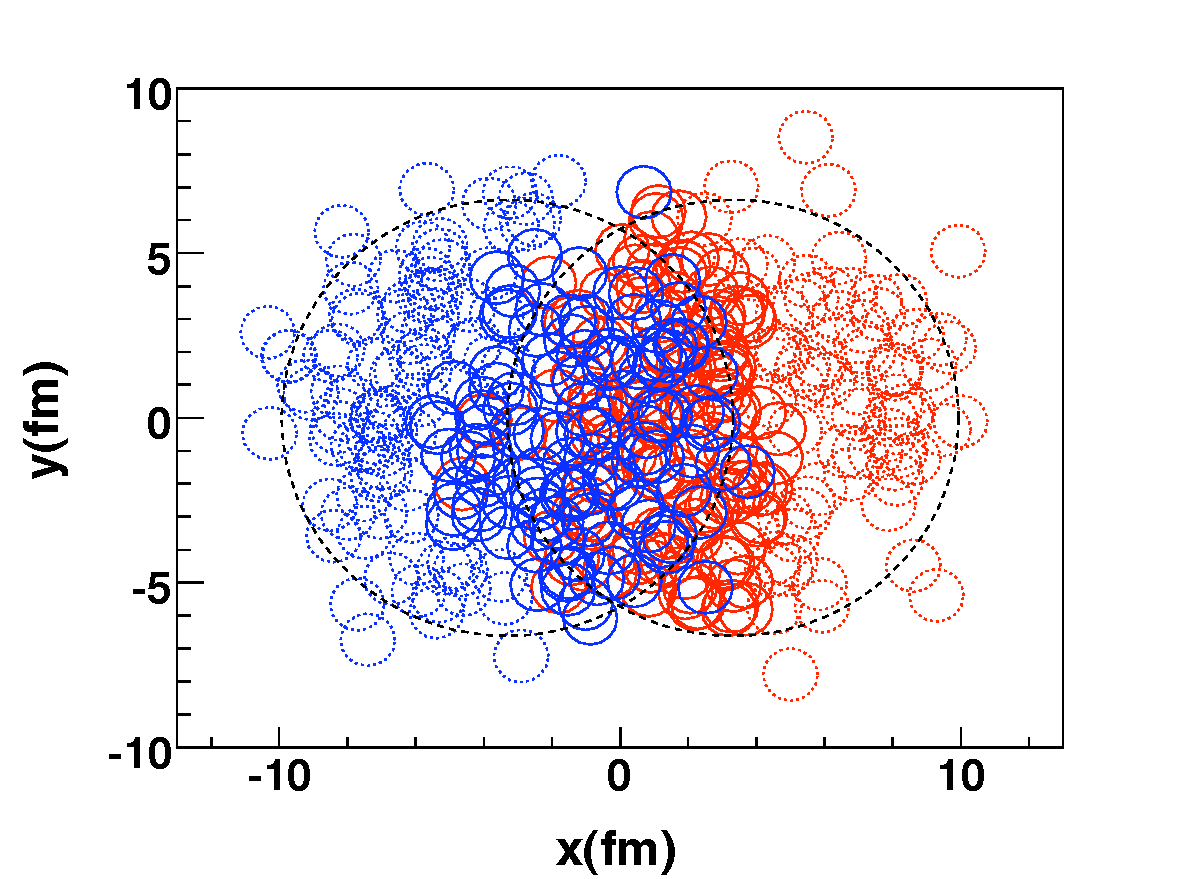
\includegraphics[width=0.75\textwidth]{figures/test_pbpb_2a}
        \caption[The result of one Glauber Monte Carlo simulation.]{The figure shows a \PbPb collision in a Glauber Monte Carlo simulation. The big circles with black dotted boundaries outline the two colliding nuclei. Small blue and red circles represent nucleons with different colours for the two nuclei. Circles with solid boundaries are participants i.e. there is an overlap with at least one nucleon from the other nucleus. Circles with dotted boundaries are spectators which do not take part in the collision~\cite{Alver:2008aq}.}
        %Permission needed?
        	\label{fig:GMC}
\end{figure}



\subsubsection{Collective motion}
\label{sec:collective}
For most cases the evolution of a heavy-ion event can be separated into four stages. A schematic illustration of the evolution of a heavy-ion collision with this division is shown in Figure~\ref{fig:HISpaceTime}. Stage 1 is the pre-equilibrium stage, the phase immediately after the collision. It is commonly assumed to last about $1\ \mathrm{fm}/c$ in proper time $\tau$. 
%Hydrodynamic description is not applicable to this regime because thermal equilibrium is not yet reached. 

\begin{figure}[htb]
\centering
               \includegraphics[width=0.75\textwidth]{pics/HISpaceTime2}
        \caption[Schematic representation of a heavy-ion collision]{Schematic representation of a heavy-ion collision as a function of time and the longitudinal coordinate $z$. The various stages of the evolution are separated by hyperbolic curves which are defined by fixed proper time $\tau=\sqrt{t^2-z^2}$. Figure from~\cite{Romatschke:2009im}.}
        %Permission needed
        	\label{fig:HISpaceTime}
\end{figure}

During the second stage the system has thermal equilibrium or at least a near-equilibrium. This lasts about $5-10\ \mathrm{fm}/c$ until the temperature of the system decreases enough for the system to lose its deconfined, strongly coupled state and hadronisation occurs. During stage 2 the matter is driven outwards by the large pressure gradient from the centre of the collision to the vacuum outside the collision volume. 

During stage 3 the hadrons still interact with each other. This ends when hadron scattering becomes rare and in the final phase hadrons become free streaming. They will move in straight trajectories until they reach the detector. 

In a heavy-ion collision the bulk collective particle production that is emitted from the QGP medium is referred to as flow. During hadronisation the pressure-driven expansion of QGP turns into the flow of mainly low-momentum particles. Since the expansion is close to isotropic the resulting particle flow is isotropic with small anisotropies of the order of $10\%$ at most. The isotropic component of flow is referred to as radial flow. Figure~\ref{fig:dndpt} shows the transverse momentum spectra $\dd N/\dd {\pt{}}$ in heavy-ion collisions. 

%In this stage hydrodynamics should be applicable if the temperature is above the deconfinement temperature~\cite{Romatschke:2009im}. 
% strongly coupled, state and hydrodynamics can no longer be used.






\begin{figure}[b!]
\centering
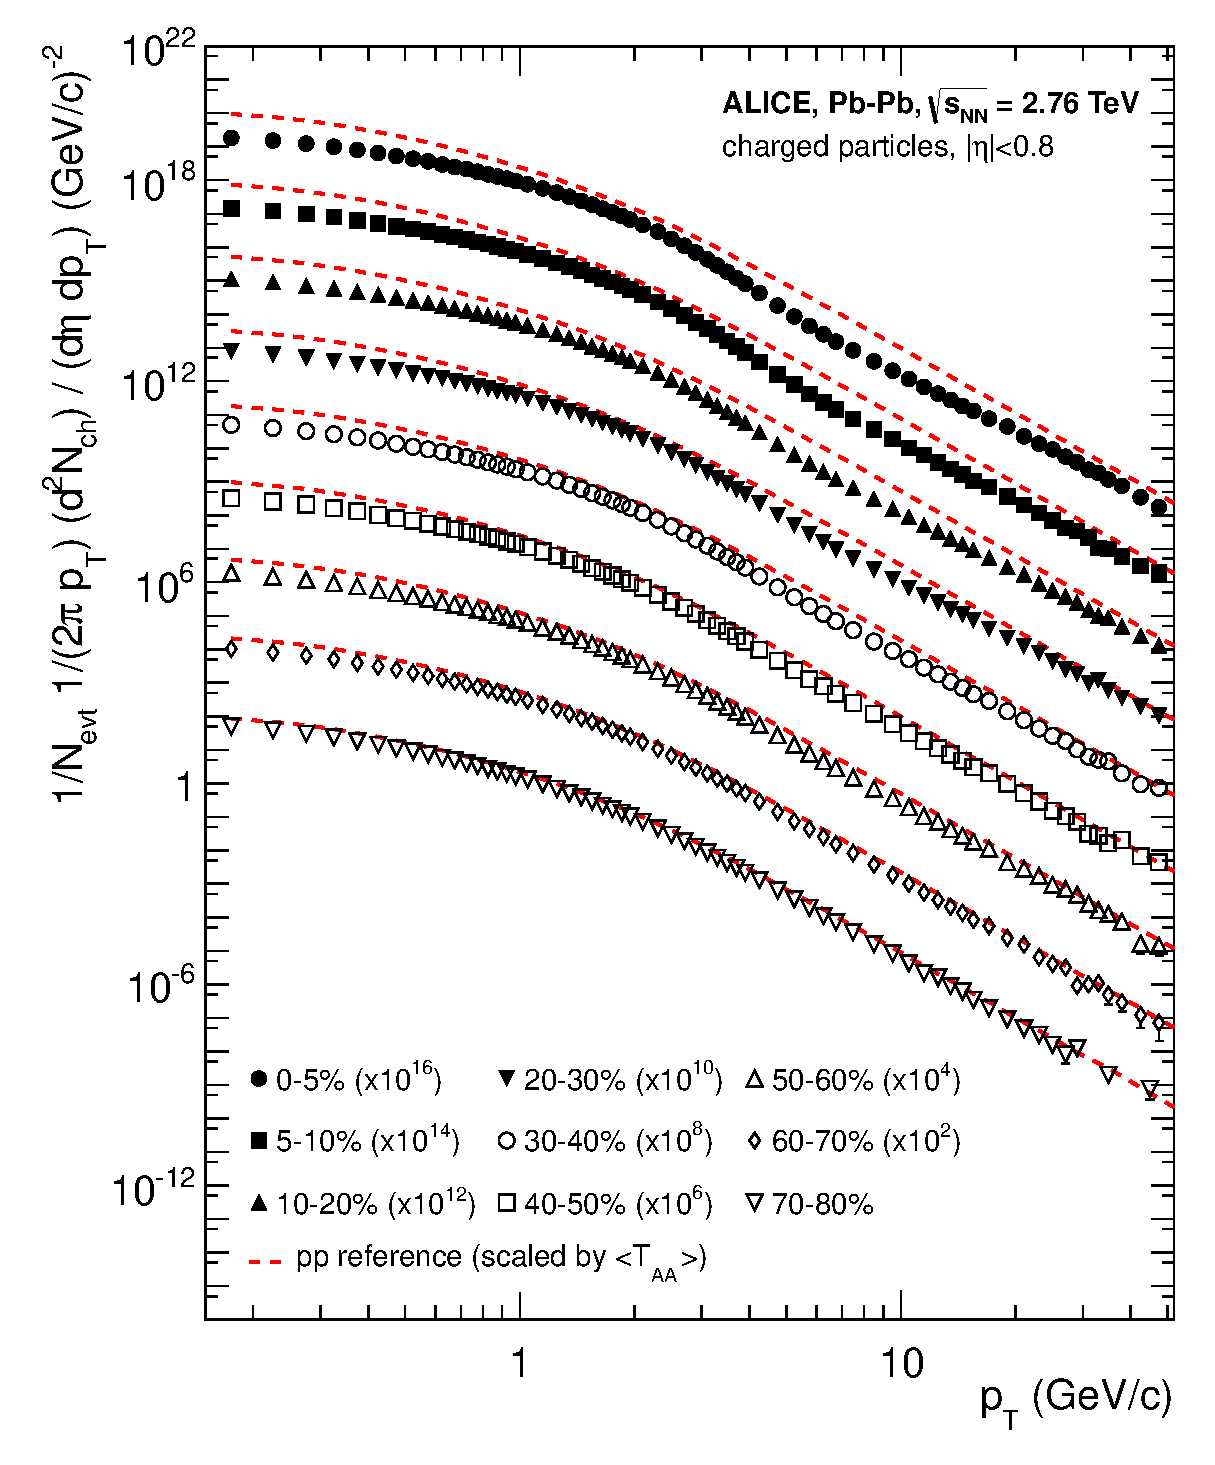
\includegraphics[width=0.6\textwidth]{pics/pT_PbPb}
\caption[Charged particle spectra]{The radial flow is represented by the charged particle spectra for different centrality classes given in the legend. The dashed lines show  proton-proton reference spectra which are scaled by the nuclear overlap function determined for each centrality class.  For clarity the distributions and the reference spectra are offset by arbitrary factors. Figure from~\cite{PRL106032301}.}
%Creative commons license
\label{fig:dndpt}
\end{figure}

%Figure~\ref{fig:dndpt} shows the transverse momentum spectra $\dd N/\dd {\pt{}}$ in heavy-ion collisions. As the vast majority of produced particles have small $\pt{}$, any observables that are integrated over $\pt{}$ are dominated by the small momentum region of the spectrum. The difference between the yield of $\unit[1]{\gevc}$ and $\unit[4]{\gevc}$ particles is already 2-3 orders of magnitude.

The geometry of the heavy-ion collision produces an anisotropic component to the collective motion. Figure~\ref{fig:flow} gives illustrations of collisions with different impact parameters. In a non-central heavy-ion collision, with a large impact parameter, the impact zone has an elliptical shape in the transverse plane. In a central collision, with a small impact parameter, the overlap region is almost circular.

\begin{figure}[b!]
\centering
        \begin{subfigure}[b]{0.52\textwidth}
                \centering
            	%\includegraphics[height=2.4in]{pics/InteractionB}
	         \includegraphics[height=2.4in]{figures/tikz/central}

                \caption{Peripheral collision}
                \label{fig:InteractionB}
        \end{subfigure}
        \begin{subfigure}[b]{0.45\textwidth}
                \centering
              % \includegraphics[height=2.4in]{pics/InteractionA}
                \includegraphics[height=2.4in]{figures/tikz/peripheral}

                \caption{Central collision}
                \label{fig:InteractionA}
        \end{subfigure}
	\caption[Illustration of flow in momentum space in central and peripheral collisions.]{Illustration of elliptic flow in central and peripheral collisions. The density of the arrows represent the strength of flow in the corresponding azimuthal direction as seen in the detectors. In a peripheral collision momentum the difference in pressure gradients gives a strong flow into the in-plane direction while the flow into the out-of-plane direction is small. In a central collision flow is more isotropic and dominated by higher harmonics. In the figure the difference is exaggerated and the difference in total multiplicity is not taken into account.}
	\label{fig:flow}
\end{figure}

During the evolution of the QGP medium this asymmetry of the impact zone is transformed into the asymmetry of particle production in momentum space. The distance from high pressure, the collision centre to low pressure, vacuum outside the impact zone varies. It is smallest in the direction of the impact parameter $\vec b$ and thus the pressure gradient is strongest in this direction, in-plane. The higher pressure gradient will produce more collective flow as compared to the out-of-plane direction~\cite{Ollitrault:1992,Ollitrault:1993, Heinz:2002}. Figure~\ref{fig:flow} illustrates the difference in impact zone and resulting flow.


Flow anisotropy is typically parametrised in the form of a Fourier composition 

\begin{equation}
E\frac{\dd{^3N}}{\dd {p^3}}=\frac{1}{2\pi}\frac{\dd {^2N}}{\pt{ }\dd {\pt{ }}\dd {\eta} } \left(1+\sum_{n=1}^{\infty}2v_n\left(\pt{},\eta\right)\cos(n(\phi-\Psi_n))\right),
%\label{eq:finalseries}
\end{equation}

\noindent where the overall normalisation, $\frac{1}{2\pi}\frac{\dd {^2N}}{\pt{ }\dd {\pt{ }}\dd {\eta} }$, gives the strength of radial flow and the coefficients $v_n$ give the relative contributions of anisotropic flow components. As in general Fourier analysis is known as harmonic analysis the components are often referred to as harmonic flow components. 
Elliptic flow, i.e. flow with two maxima, is represented by $v_2$ and $v_3$ represents triangular flow while the first coefficient, $v_1$, is connected to directed flow~\cite{Voloshin:1994mz}. Because of momentum conservation directed flow is in total assumed to be zero. In certain rapidity or momentum regions it can be nonzero but it must be canceled by other regions.

In a peripheral collision $v_2$ is the dominant part of anisotropic flow as it arises from the asymmetric geometry of the collision region.  For a long time the odd harmonics were considered to be negligible, because they would require a more complex asymmetry. In 2007 Mishra {\emph et al.}~\cite{Mishra:2007tw} argued that inhomogeneities in the initial state density would lead to non-zero $v_n$ values for $v_3$ and other higher harmonics. As the colliding nuclei are not static objects, the arrangement of the nucleons at the time of a collision is random~\cite{Alver:2010gr}. Therefore the shape of the collision zone is not symmetric but rather more complex. On the other hand, inside the collision zone the created medium is not homogenous. Instead the medium includes hot spots with higher density. It is expected that higher harmonics of $v_n$ would be suppressed more by viscous effects and thus the shape of $v_n$ as a function of $n$ could be used to study $\eta/s$~\cite{Mocsy:2010um}.

The first one to predict anisotropic flow in heavy-ion collisions was Ollitrault in 1992~\cite{Ollitrault:1992} and the first experimental studies were conducted in 1993 at the AGS~\cite{PhysRevLett.70.1393}. Instead of the Fourier composition these initial studies used alternative approaches. In AGS the reaction plane angle in one rapidity region was observed to be correlated with the particle production in another rapidity region. The first ones to introduce the Fourier decomposition were Voloshin and Zhang in 1996~\cite{Voloshin:1994mz}.


\begin{figure}[tb]
	\centering
	\begin{subfigure}[t]{0.5\textwidth}
                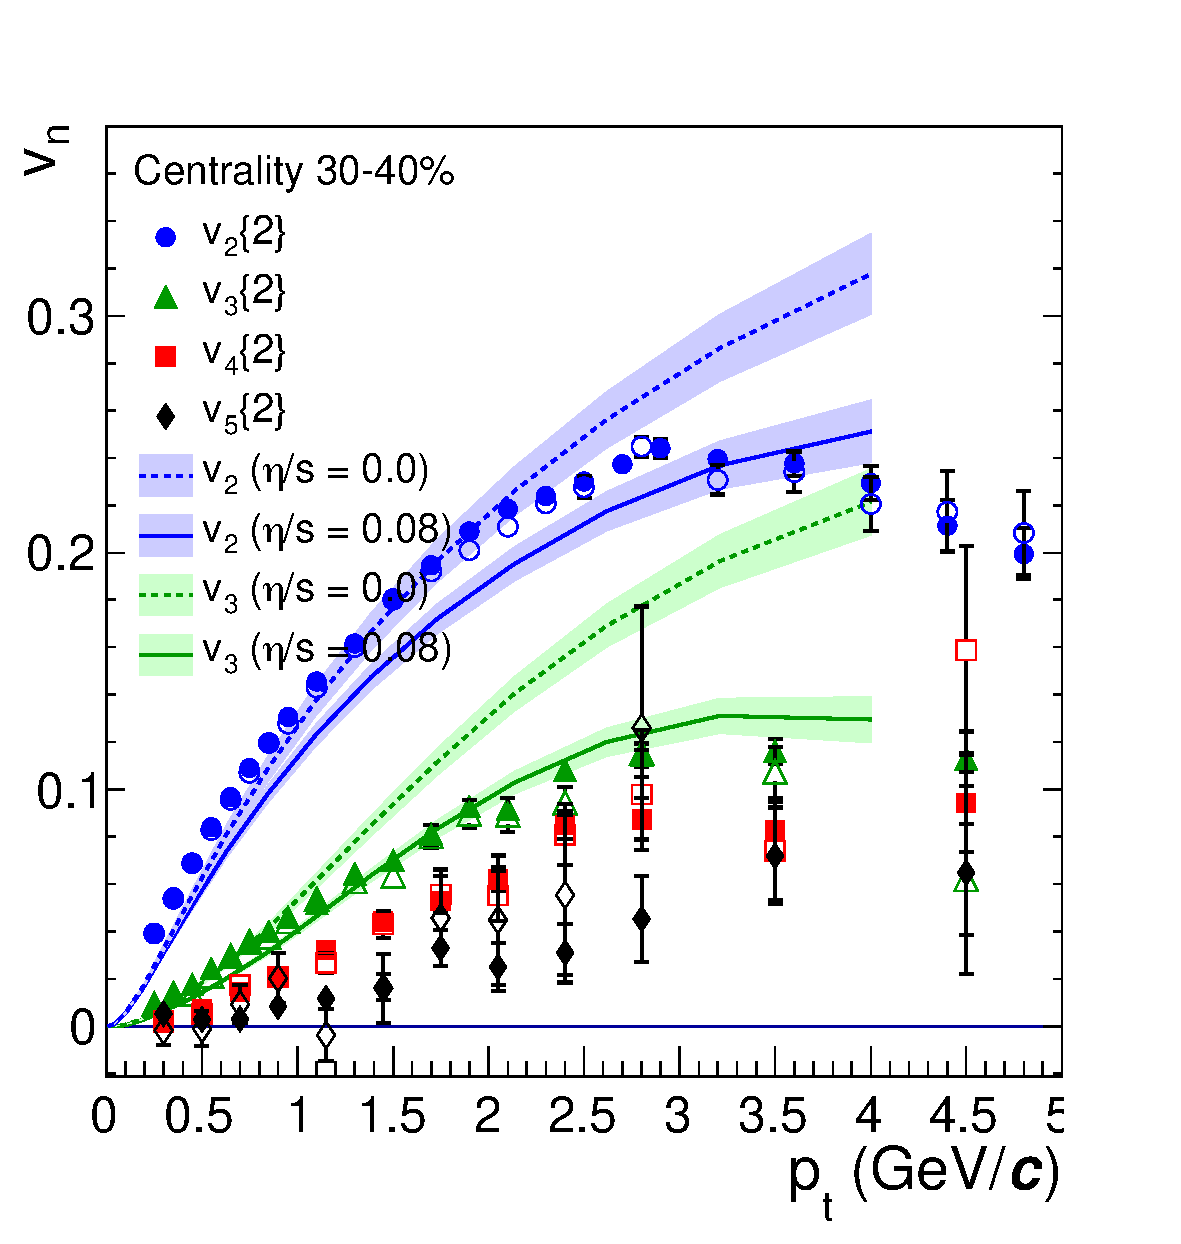
\includegraphics[width=\textwidth]{pics/alice_vn_figa.pdf}
        %\caption[ALICE measurement of $v_2$, $v_3$, $v_4$, $v_5$]{ALICE measurement of $v_2$, $v_3$, $v_4$, $v_5$ as a function of transverse momentum. The flow coefficients are determined by two-particle correlations using different rapidity separations.  The full and open symbols are for $\Delta\eta > 0.2$ and $\Delta\eta > 1.0$. The results are compared to hydrodynamic predictions~\cite{Schenke:2011tv} with different values of $\eta/s$~\cite{PRL107032301}.}
        \label{fig:higherharmonics}
        \end{subfigure}
        \quad
        \begin{subfigure}[t]{0.45\textwidth}
        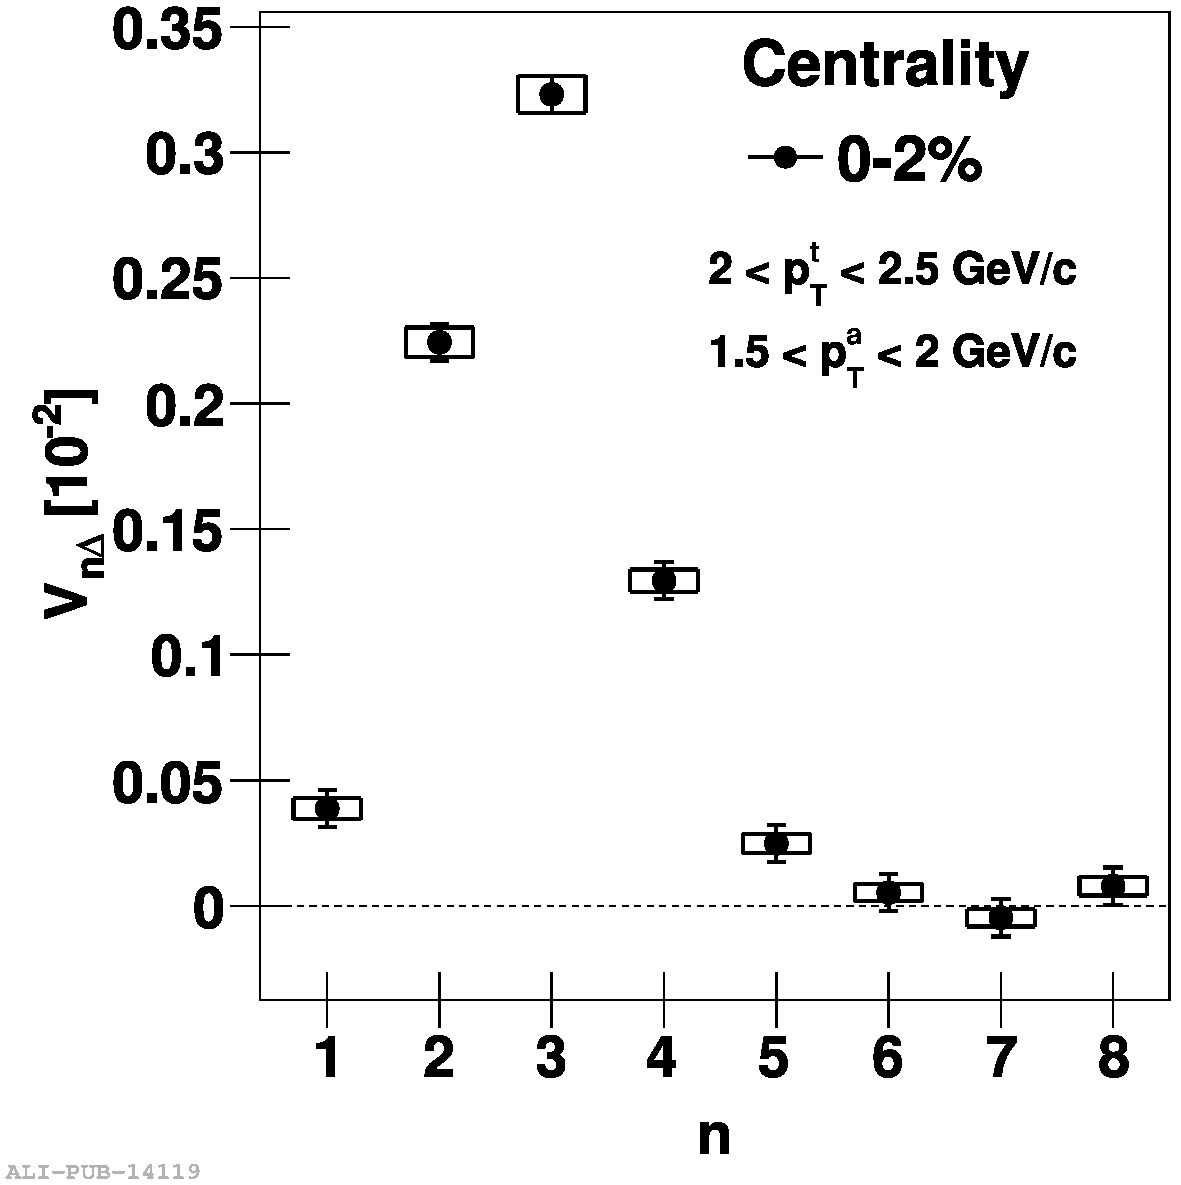
\includegraphics[width=\textwidth]{pics/2012-Jun-06-fig02b}
       % \caption{Amplitude of $v_n$ harmonics as a function of $n$ for the 2\% most central collisions as  measured by ALICE~\cite{Aamodt2012249}.}
        \label{fig:alicepowers}

        \end{subfigure} 
        
%        \begin{subfigure}[t]{\textwidth}
 %               \includegraphics[width=\textwidth]{pics/atlas_powerspectra.png}
%        \caption{Power spectra of $v_n$ for the 1\% most central collisions measured by ATLAS~\cite{PhysRevC.86.014907}.}
%        \label{fig:atlaspowers}
 %       \end{subfigure}
                \caption[Flow measurements of higher harmonics]{Flow measurements of higher harmonics. \emph{left:} ALICE measurement of $v_2$, $v_3$, $v_4$, $v_5$ as a function of transverse momentum. Two-particle correlations are used to obtain the harmonic coefficients. The full and open symbols are for different $\Delta\eta$ separation between the particles ($\Delta\eta > 0.2$ and $\Delta\eta > 1.0$). The observations are compared to hydrodynamic calculations~\cite{Schenke:2011tv} with varying values of the shear viscosity to entropy ratio $\eta/s$. Figure from~\cite{PRL107032301}. \emph{right:} Amplitude of $v_n$ coefficients as a function of $n$ for the 2\% most central collisions as measured by ALICE. Figure from~\cite{Aamodt2012249}. }
                %Creative commons license
                \label{fig:vnpowers}

\end{figure}


Figure~\ref{fig:vnpowers} shows measurements of different harmonics coefficients. The left panel shows the flow coefficients in peripheral collisions as a function of track $\pt{}$ as measured by ALICE~\cite{PRL107032301}.  As shown on the right hand panel of Figure~\ref{fig:vnpowers} the $v_n$ values decrease in central collisions as a function of $n$ for $n>3$. In peripheral collisions the elliptic flow component $v_2$ will be larger.

In Figure~\ref{fig:vnpowers} the results are compared to predictions from hydrodynamic calculations~\cite{Schenke:2011tv}. In general the measured collective flow in heavy-ion collisions has been successfully modelled with the relativistic version of hydrodynamics. The power of this approach lies in its simplicity and generality. Hydrodynamic calculations only require that the system reaches at least local thermal equilibrium. For this the system must have a mean free path that is shorter than the length scales of interest, which is assumed to hold for the strongly coupled QGP phase of a heavy-ion collision~\cite{Romatschke:2009im}.

The first approaches using the relativistic version of hydrodynamics were performed already in the 1950's~\cite{Landau:1953gs}, before QCD was discovered. The early studies used it to model proton-proton collisions. For the use of heavy-ion collisions hydrodynamics has been under development since the 1980's. One early example is the study of boost-invariant longitudinal expansion and infinite transverse flow by Bjorken~\cite{PhysRevD.27.140}. Later studies added finite size and dynamically generated transverse size~\cite{Baym:1984sr, PhysRevD.34.794}. 

%Major steps were taken later with the addition of finite size and and dynamically generated transverse size~\cite{Baym:1984sr, PhysRevD.34.794}, a part of which was done at the University of Jyväskylä. %The role of hydrodynamics in heavy-ion physics was strengthened when QGP was observed to behave like a liquid by RHIC~\cite{Adcox:2004mh}. 

Over the years understanding of the properties of the QGP has been improved with the help of new data from LHC and RHIC and theoretical developments.
For example, as shown in Figure~\ref{fig:etasT}(a), the quantification of the temperature dependence of the shear viscosity over entropy ratio, $\eta/s$ has been tested with an event-by-event model~\cite{Niemi:2015qia} that combines viscous hydrodynamic calculations with the Eskola-Kajantie-Ruuskanen-Tuominen (EKRT) model for initial conditions.
%event-by-event Eskola-Kajantie-Ruuskanen-Tuominen (EKRT) + viscous hydrodynamic calculations~\cite{Niemi:2015qia}, where the first qualitative possibilities of the dependence were investigated.

The initial density profiles for hydrodynamic simulations are calculated using a next-to-leading order perturbative-QCD (pQCD) and the EKRT model~\cite{Paatelainen:2012at,Paatelainen:2013eea}. The following space-time evolution is described by relativistic dissipative fluid dynamics. The simulation is performed using different parametrisations of the temperature dependence of the shear viscosity to entropy density ratio $\eta/s(T)$. 

This model has been observed to give a good description of the charged hadron multiplicity and of the low-\pt{} region of the charged hadron spectra both at RHIC and at LHC~\cite{Niemi:2015qia}. Each of the different $\eta/s(T)$ parametrisations were adjusted to reproduce the measured $v_n$ from central to mid-peripheral collisions.
Previous measurements~\cite{ALICE:2016kpq} have ruled out models where the temperature of the phase transition is larger than for "param1".
The two sets of parameters which described most of the data are labeled as "best fits" in Figure~\ref{fig:etasT}(a).
For the "param1" parametrisation the phase transition from the hadronic to the QGP phase occurs at the lowest temperature, around 150~MeV. This parametrisation is also characterised by a moderate slope in $\eta/s(T)$ which decreases (increases) in the hadronic (QGP) phase.

The estimation of the $\eta/s(T)$ dependence has been also studied with a Bayesian analysis, which is applied to form the initial conditions with no assumptions on the physical mechanisms of entropy production~\cite{Bernhard:2016bar}. The robust statistical analytical methods allow calibrating the model to data in a multi-dimensional parameter space. In addition to finding the most likely combination of input parameters, the Bayesian statistical method provides the full uncertainty quantification in the form of posterior probability distributions for all the parameters. The $\eta/s(T)$ parametrisation resulting from this analysis is shown in Figure~\ref{fig:etasT}(b).

\begin{figure}
       \begin{overpic}[width=0.45\textwidth]{figures/etapers_bestfit.pdf}
         \put(10,82){\tiny H. Niemi, K.J. Eskola, R.Paatelainen}
         \put(10,78){\tiny (Phys. Rev. C 93, 024907 (2016), arXiv:1505.02677)}
        \end{overpic}
        \begin{overpic}[width=0.55\textwidth]{figures/region_shear.pdf}
         \put(9,70){\tiny Steffen A. Bass et. al, Global Bayesian Analysis}
          \put(9,67){\tiny (Nucl.Phys. A967 (2017) 67-73 , arXiv:1704.07671)}
          \put(15,35){\small(b)}
        \end{overpic}
        \caption{Temperature dependence of $\eta/s$. \emph{left:} Different parametrisations of $\eta/s(T)$ that have been tested in hydrodynamical simulations. Figure from~\cite{Niemi:2015qia}. \emph{right:}  Result of a global Bayesian analysis narrowing down the possible $\eta/s(T)$ behaviour. Figure from~\cite{Bernhard:2016bar}.}
        \label{fig:etasT}
        '%Permission needed for a) and b)
 \end{figure}

Based on these model calculations, the phase transition from the hadronic to the QGP phase occurs at the lowest temperature, around 150~MeV.
Although the temperature dependence of the $\eta/s$ is still not well established, the calculations generally suggest a minimum value of $\eta/s$~from 0.08 to 0.12, close to the universal limit $1/(4\pi)$~\cite{Kovtun:2004de}.

Recently, several advancements have been made in order to further constrain the temperature dependence of $\eta/s$. New observables, such as the symmetric cumulants~\cite{ALICE:2016kpq,Acharya:2017gsw}, have provided detailed information on the temperature dependence over the evolution of the QGP. Furthermore, the non-linear formalism has resulted in remarkable new constraints on the initial conditions~\cite{Acharya:2017zfg}, and the $\eta/s$ at the freeze-out conditions, which is among the least understood parts of hydrodynamic calculations.


%Comparing hydrodynamical calculations to experimental results has provided a path to studying the $\eta/s$ value of QGP. 












